

\chapter{Réalisation et tests}
\section{Introduction}
Après avoir exposé en détail notre méthode automatique d'élagage dans le chapitre précèdent, nous discuterons maintenant sur les technologies et outils qui ont été choisis pour matérialiser cette approche et garantir son déploiement efficace. De ce fait, il est essentiel d'examiner en détail les langages de programmation, les bibliothèques et les frameworks qui ont été sélectionnés pour concrétiser notre approche. Nous offrons également un aperçu des stratégies de test que nous avons employées pour évaluer la performance de notre solution. Ces tests ont été établis pour mesurer les performances des modèles VGG-19 et ResNet-34 et la précision de chacun.

\section{Modèles et jeu de données utilisés}



\section{Technologies utilisées}
\subsection{Python}

\begin{figure}[hbt!]
  \centering
  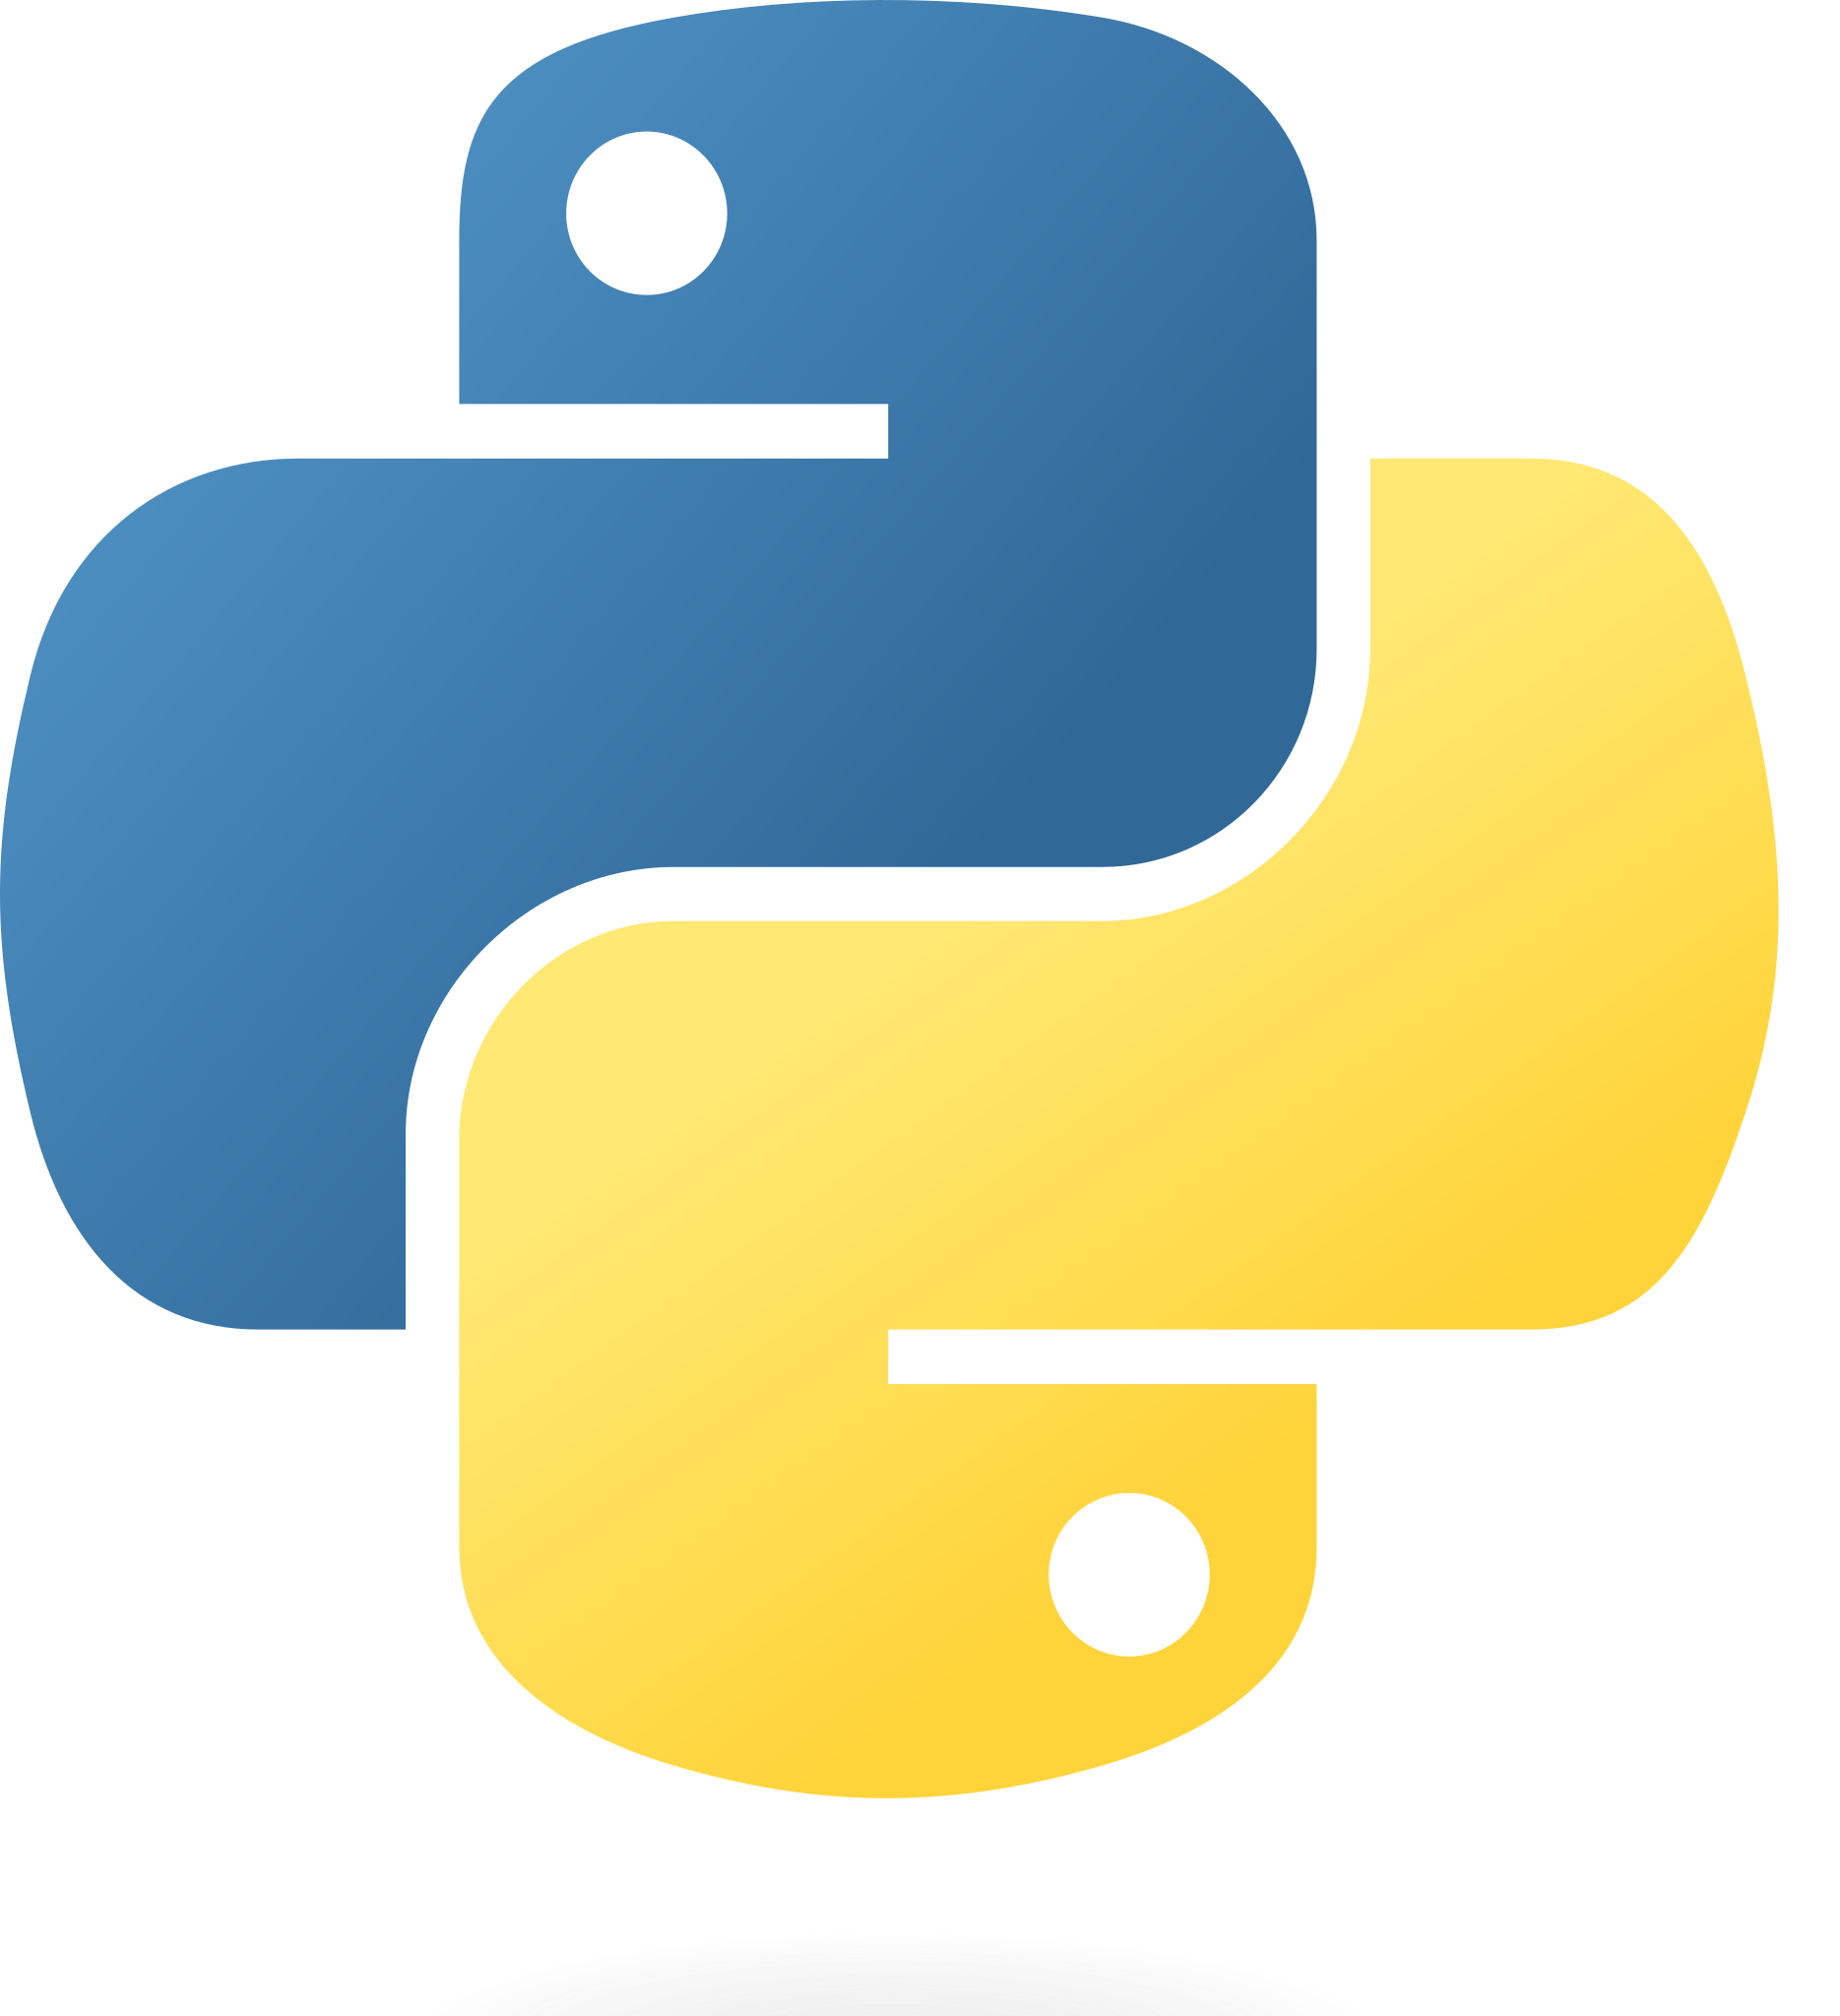
\includegraphics[width=4cm]{images_pfe/python.png}
  \caption{Python.}
  \label{fig:python}
\end{figure}
\FloatBarrier
\medskip

Python joue un rôle important dans le domaine de l'intelligence artificielle (IA) grâce à sa polyvalence, sa simplicité et sa richesse en bibliothèques spécialisées. En tant que langage de programmation, Python est devenu le premier choix  pour de nombreux chercheurs, ingénieurs et développeurs travaillant dans le domaine de l'IA. D'une part, Python est connu pour sa syntaxe claire et lisible, ce qui  permet aux nouveaux arrivants dans le domaine de l'IA de se familiariser rapidement avec les concepts de base. D'autre part, Python offre plusieurs bibliothèques et frameworks spécialisés dans l'IA, tels que TensorFlow, Keras, PyTorch et Scikit-learn. Ces bibliothèques sont souvent utilisées pour le développement de réseaux de neurones, d'algorithmes d'apprentissage automatique et d'autres techniques d'IA. Finalement, Python est un langage polyvalent qui permet aux développeurs de créer et tester différentes approches rapidement.

\section{Bibliothèque utilisées}
Python offre une riche collection de bibliothèques spécialisées dans plusieurs domaines, en particulier l'IA. Ces bibliothèques offrent des outils et des frameworks puissants pour développer des modèles d'apprentissage automatique, des réseaux de neurones, et bien plus encore. Dans cette section, nous allons explorer les bibliothèques que nous avons utilisé pour implémenter et tester notre méthode.
\subsection{NumPy}

\begin{figure}[hbt!]
  \centering
  
\includegraphics[width=4cm]{images_pfe/numpy.png}
  \caption{NumPy.}
  \label{fig:numpy}
\end{figure}
\FloatBarrier
\medskip

NumPy \footnote{acronyme de "Numerical Python"} est une bibliothèque open source qui offre de nombreuses fonctionnalités pour le calcul numérique en Python. Elle offre un support puissant pour la manipulation de tableaux multidimensionnels, ainsi que pour l'exécution de calculs mathématiques complexes sur ces tableaux. Ces tableaux multidimensionnels permettent de stocker et de manipuler efficacement des données numériques sous forme de matrices et de vecteurs. Elle fournit également des fonctions mathématiques de base, des opérations d'algèbre linéaire, des opérations sur les tableaux, des fonctions statistiques et bien plus encore. Elle est largement utilisé en IA pour le traitement et la manipulation de données, la préparation de jeux de données, ainsi que pour la mise en œuvre d'algorithmes d'apprentissage automatique et de réseaux de neurones. La performance élevée de NumPy en calcul numérique en fait un bon choix pour les tâches intensives en termes de calcul.


\subsection{Matplotlib}
\begin{figure}[hbt!]
  \centering
  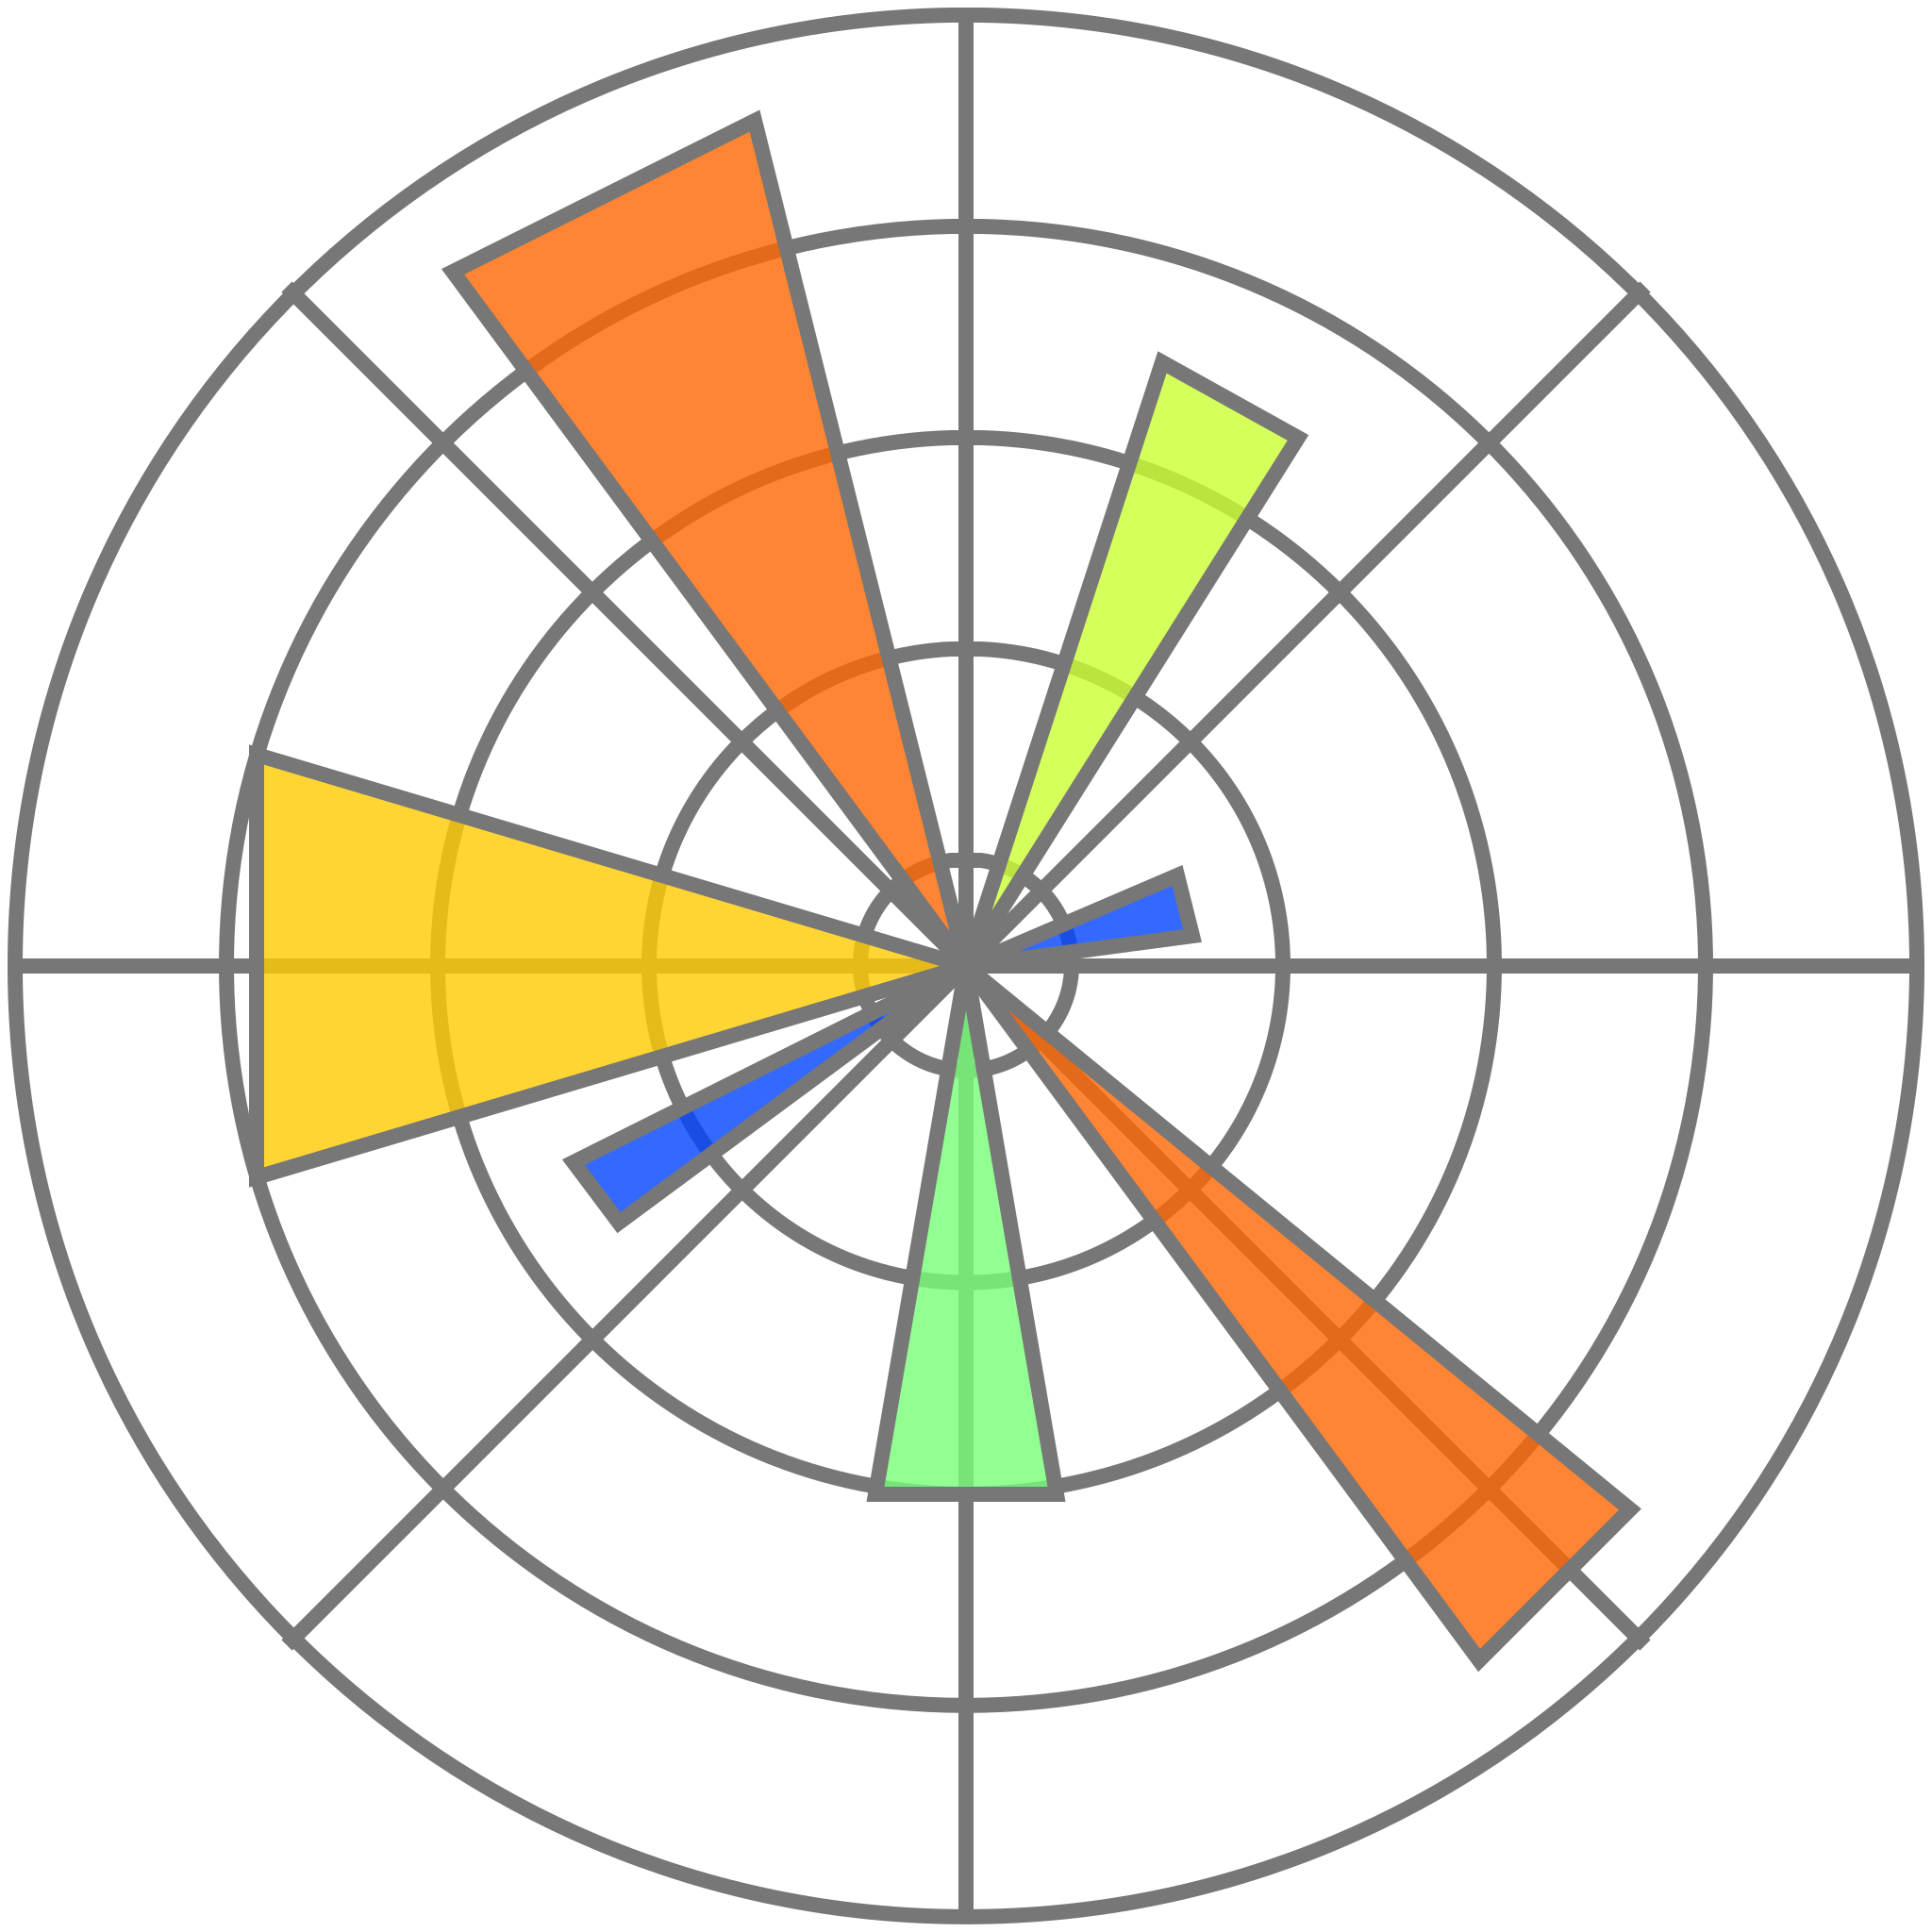
\includegraphics[width=4.5cm]{images_pfe/matplotlib.png}
  \caption{Matplotlib.}
  \label{fig:matplotlib}
\end{figure}
\FloatBarrier
\medskip

Matplotlib est une bibliothèque de visualisation en Python qui aide à créer des graphiques et des visualisations de données de manière interactive et statique. Cette bibliothèque offre un large éventail d'outils pour générer des graphiques de haute qualité à partir de données numériques. Son objectif est de permettre aux utilisateurs de représenter visuellement des données complexes de manière claire et compréhensible. Pour cela, elle propose une grande variété de types de graphiques, tels que les graphiques linéaires, les graphiques en barres, les graphiques à secteurs, les graphiques de dispersion, les graphiques 3D, etc. Elle permet également de personnaliser presque tous les aspects des graphiques, y compris les étiquettes, les couleurs, les styles de ligne, les titres, les axes et les légendes. L'utilisation de Matplotlib est essentielle dans l'analyse de données, la science des données et la recherche en général. En intelligence artificielle et en apprentissage automatique, Matplotlib est souvent employé pour visualiser les performances des modèles, les distributions de données, les tendances, les caractéristiques importantes, les matrices de confusion, les courbes d'apprentissage, etc.

\subsection{Pytorch}

\begin{figure}[hbt!]
  \centering
  
\includegraphics[width=4cm]{images_pfe/pytorch.png}
  \caption{Pytorch.}
  \label{fig:pytorch}
\end{figure}
\FloatBarrier
\medskip

PyTorch est une bibliothèque open-source d'apprentissage automatique et d'intelligence artificielle en Python, développée principalement par Facebook's AI Research lab (FAIR). Elle repose sur un concept fondamental appelé "tenseur", qui est une structure de données multidimensionnelle similaire aux tableaux NumPy et elle est conçue pour faciliter le développement et la mise en œuvre de modèles de réseaux de neurones profonds. PyTorch est surtout distinguée par sa prise en charge des calculs automatiques de gradients, ce qui signifie qu'il est possible de définir des opérations mathématiques sur les tenseurs et que PyTorch peut automatiquement calculer les gradients de ces opérations qui sont nécessaires pour ajuster les poids dans les réseaux de neurones et ainsi minimiser une fonction de perte. Elle est utilisé pour la conception des modèles de réseaux de neurones profonds, y compris les réseaux de neurones convolutionnels (CNN), les réseaux de neurones récurrents (RNN), les transformeurs, etc.

\subsection{Torchvision}

\begin{figure}[hbt!]
  \centering
  
\includegraphics[width=4cm]{images_pfe/torchvision.png}
  \caption{Torchvision.}
  \label{fig:torchvision}
\end{figure}
\FloatBarrier
\medskip

Torchvision est une bibliothèque qui fait partie de PyTorch. Elle est spécifiquement conçue pour faciliter le chargement et la transformation de jeux de données d'images couramment utilisés dans le domaine de l'apprentissage automatique et de la vision par ordinateur. Elle offre des outils pour prétraiter les données d'image, créer des ensembles de données, appliquer des transformations aux images et charger des ensembles de données préexistants. Elle propose des classes pour charger facilement des ensembles de données standard tels que MNIST, CIFAR-10, ImageNet, etc. Elle permet également d'appliquer diverses transformations aux images, telles que le redimensionnement, le recadrage, la normalisation, les rotations, les miroirs, etc. qui sont utiles pour augmenter la variabilité des données.

\subsection{NNI}

\begin{figure}[hbt!]
  \centering
  
\includegraphics[width=6cm]{images_pfe/nni.png}
  \caption{NNI (Neural Network Intelligence).}
  \label{fig:nni}
\end{figure}
\FloatBarrier
\medskip

NNI (Neural Network Intelligence) est une bibliothèque open-source développée par Microsoft Research. Elle fournit un ensemble d'outils et de bibliothèques pour faciliter l'exploration et l'optimisation des espaces d'hyperparamètres, ainsi que pour la recherche automatique d'architectures de modèles. Elle permet aux utilisateurs de définir un espace de recherche pour les hyperparamètres, tels que les taux d'apprentissage, les tailles de lot, les architectures de couches, etc. NNI exécute ensuite des expériences en utilisant différentes configurations d'hyperparamètres et rapporte les résultats, y compris les performances du modèle. Elle est très utile dans le domaine de l'apprentissage automatique, car elle simplifie et automatise le processus d'ajustement des hyperparamètres et d'exploration des architectures, ce qui peut considérablement accélérer le développement de modèles performants.

\section{Outils utilisés}

\subsection{Google Colab}

\begin{figure}[hbt!]
  \centering
  
\includegraphics[width=7cm]{images_pfe/colab.png}
  \caption{Google Colab.}
  \label{fig:colab}
\end{figure}
\FloatBarrier
\medskip

Google Colab (abrégé de Colaboratory) est une plateforme de notebooks interactifs basée sur le cloud, développée par Google. Elle permet aux utilisateurs d'écrire, d'exécuter et de partager du code Python de manière collaborative, sans nécessiter de configuration ou d'installation. Elle propose des notebooks interactifs qui permettent d'insérer des cellules de code exécutable et des cellules de texte et chaque notebook Colab s'exécute dans un environnement virtuel où les utilisateurs peuvent accéder à la puissance de calcul des processeurs graphiques (GPU) et des unités de traitement tensoriel (TPU) pour accélérer l'entraînement de modèles d'apprentissage automatique. Elle propose également de nombreuses bibliothèques préinstallées, mais les utilisateurs peuvent également installer et utiliser des bibliothèques tierces via des commandes simples.

\subsection{Google Drive}

\begin{figure}[hbt!]
  \centering
  
\includegraphics[width=6cm]{images_pfe/drive.png}
  \caption{Google Drive.}
  \label{fig:drive}
\end{figure}
\FloatBarrier
\medskip

Google Drive est un service de stockage en ligne développé par Google pour stocker, synchroniser et partager des fichiers et des dossiers sur le cloud. Il offre une variété de fonctionnalités telles que le stockage en ligne, la synchronisation multi-appareils, le partage de fichiers, la collaboration en temps réel, etc. De plus, il peut être utilisé avec Google Colab.

\section{Tests et résultats}

\section{Conclusion}
